\documentclass[../main.tex]{subfiles}

\begin{document}

To understand how segregation occurs in a system, we have to look at how the decisions of the individual parts of the system affect the system as a whole. In other words, we have to look at the emergent properties of the system. In this chapter, we will see what complex systems and emergent properties are. We will try to give a definition to segregation, look at computational models, at what they are and how they are being used to accelerate scientific discovery. Then, we will look at a particular set of computational models: the agent-based model. Schelling's segregation model is an agent-based model, but before we will discuss in detail Schelling's model in the next chapter, we will look here at a slightly different model: the multi-agent bargaining model. This will give us a better understanding of how agent-based models work and why they are so important. Next, we will look at a few papers that were influenced by Schelling's model and finally, we will talk about the technical tools we chose to construct our computational model and the reasoning behind our choices.

\subsection{Emergent Properties}

In philosophy, \textbf{emergence} refers to the process where certain patterns or regularities arise from the interaction of smaller identities that do not exhibit such properties. When we talk about \textbf{emergent property} we refer to a property that a system or a collection has, but which does not characterise the individual parts of the system. In other words, we apply the term "emergent" to certain properties of the whole complex system. Such a complex system is, for example, the brain with neurons representing the individual parts, or the Earth's global climate is also seen as a complex system. 

It is generally agreed that not all properties of a system are emergent properties. But what makes a property \textit{emergent}? Mark Bedau in \textit{Weak Emergence}\cite[]{bedau_weakEmergence} says that a property is to be considered an emergent property if it is both \textit{autonomous} and \textit{constituted} by the underlying processes. It is important that both properties are met simultaneously. Being just constituted by the underlying processes, \verb|i.e.| not autonomous, would not differentiate this property from any resultant property. For example, the weight of a system is calculated by adding up the weight of the individual parts of the system, but it is not autonomous. 

In 2003 in \textit{Downward Causation and the Autonomy of Weak Emergence}\cite[]{bedau_downwardCausation}, Bedau mentioned a third criterion that should be considered: the property needs to be relevant to scientific practice. In the article \textit{Simulation-Based Definitions of Emergence}\cite[]{baker_defEmergence}, Alan Baker states that this vague criterion "has led to a focus on the cluster of approaches including neural networks, agent-based models, and dynamical systems theory which has come to be referred to collectively as complexity science".

Thus, the notion of "emergence" can be subdivided into two categories: \textbf{weak emergence} and \textbf{strong emergence}. The weak emergence is a type of emergence where the emergent property can be simulated by computers. On the other hand, a strong emergence is an older notion and it implies that the emergent property cannot be simulated computationally.


Bedau [\citeyear[]{bedau_downwardCausation}] has the following definition of weak emergent: Given a system and a property P of the system, P is weak emergent if and only if P is delivered from all the system's micro facts but \textit{only} by simulation. Although the idea of a simulation is well-understood, the line between an emergent property that can be deduced only by simulation and an emergent property that can be derived, predicted or explained from a present state is unclear. In his article for the \textit{Journal of Artificial Societies and Social Simulation, Volume 13} [\citeyear[]{baker_defEmergence}], Alan Baker addresses this issue. He explores the epistemological ramification of the definition by trying to answer questions, such as: How and when emergent properties can be predicted? Without clear boundaries between simulation based and non-simulation based techniques, the definition does not hold. Baker also emphasises how challenging it is to define such boundaries. Hence, tracing a path between weak emergent and strong emergent is not trivial. However, in both cases, weak and strong emergence, we are interested in studying the new properties that emerge once the system gets larger, properties that are not shared by the individual components of the system and do not appear at a previous state. We are interested in how the interaction of each individual part with its immediate surroundings causes a chain of processes that can lead to some kind of pattern or order in the final state. And we are also interested in the role the simulation has.

\subsection{Computational models in social sciences}
Experiments run by economists and social psychologists and the study of history has shown that human motivations are not entirely self-regarding, they are influenced by others around us and in many cases, we can notice the existence of sacrifice towards a common, larger objective. And although, so far, group effects were the focus of empirical studies by historians, economists and other social scientists, in order to understand how individuals choose their preferences, it is necessary to analyse both the individual and the group interaction. Evolutionary Game Theory is just one example that focuses on the individual, using agent-based models. Furthermore, formal evolutionary models do not take into account the fact that human groups are highly segregated, and in many cases the segregation happens intentionally. The individual interaction is almost never random when it comes to his or her preferences. 

In this section, we are going to look at the definition of segregation and then we are going to argue \textbf{the need of computational models in general and the agent-based models in particular}. We are going to look into detail to the pros and cons of an agent computation and we will mention different types of agent-based models.


\subsubsection{Segregation Overview}
\textbf{Segregation} may refer to a separation of people based on their ethnicity, race, sex, religion, geographic location, housing, occupation, economic status, age, etc., or a separation of objects, for example, segregation of materials or particle segregation. We are going to focus on \textit{racial segregation}. However, the agent-based model that we are going to discuss in this project can be applied to any type of segregation, for any two types of agents (a type A and a type B).

Racial Segregation is the separation of humans into ethnic or racial groups in daily life. It may apply to activities such as eating in a restaurant, drinking from a water fountain, using a public toilet, attending school, going to the movies, riding on a bus, or in the rental or purchase of a home\cite[]{segregation}. Thomas Schelling was one of the first scientists to address Racial Segregation and present a social dynamics model.

With a few exceptions, throughout the history, wherever there have been multiracial citizens, there has been racial segregation. An example of racial segregation in our history could be the 35 acts by Kilkenny in 1366 (The Statutes of Kilkenny) which were forbidding English settlers in Ireland to marry Irish people, adopt Irish children or even have Irish names. We could also mention the continuous battle between whites and blacks in the United States of America. Throughout history, there are plenty of examples where the separation between the people of the two different colour groups in the USA was very clear: we talking about different lanes for movie theatres, different restaurants or housings for white and blacks. Another, more tragic example of racial segregation is the Nazi Germany(1933-1945). Nazi started a \textit{racial hygiene programme} by compulsory extermination of Untermenschen ("sub-humans"). They labelled Jews and Romani (or Gypsies) and persons of colour as inferior, inhuman and thus unworthy of life. \cite[]{nazi}

Sadly, segregation is still a big issue in nowadays society. We could mention here an example of segregation as recent as 2007. On 28 April 2007, in Bahraini (officially the Kingdom of Bahrain, an island country), the lower house of Parliament passed a law banning unmarried migrant workers from living in residential areas. \cite[]{bahraini}

Even looking at the United Kingdom, which has numerous laws that demand racial equality, due to a large number of cultural differences between communities, racial segregation has emerged in some parts of the country. The separated communities are largely representative of Indians, Pakistanis, and other sub-continentals. The segregation is thought to have occurred due to the ethnic tension, and deterioration of the standard of living, levels of education and employment among ethnic minorities in poorer areas. This type of racial segregation can be noticed in particular in residential areas. There is an indication of a market preference amongst the more wealthy to reside in areas of less ethnic mixture.\cite[]{segregation} This is something that we are going to analyse: how minor local preferences can lead to large segregation patterns in the system.  Thus, we will get an understanding of just why it is so hard to combat racial segregation.


\subsubsection{Computational models in general}
We are surrounded by complex systems, from atoms which spontaneously form molecules to plants, animals, fungi, physical conditions etc. which form ecosystems and to humans that form societies.  Social scientists have always been interested in solving the mysteries of these systems, in analysing their behaviours. However, these are in most cases complex, nonlinear systems which cannot be simply analysed using simple-logic or other intuitive analytical solutions. The evolution of computers opens new doors for us, allowing us to experiment on a model with different variables. This allows us to simulate a wide range of scenarios, avoiding the need of deriving a mathematical analytical solution. A computational model uses a large number of variables with each representing a characteristic of the system. \\

\textbf{Accelerating scientific discoveries through computational modeling}

Computational modelling allows scientists to run thousands of simulated- experiments in a relatively short amount of time; in many cases they are run simultaneously. This way, researchers can quickly identify the physical experiment that is most likely to help them to solve the problem they are working on.

Lets look at an example so we could understand better how computational modeling can save not only time, but also resources when trying to find a new solution or to improve an existing one. Assume that a bakery is trying to come up with a cake composition that would be dense enough to support a multiple level cake for special occasions like weddings. They want it to be solid enough so it would not fall during transportation and keep all the ornaments attached in place, but they do not want to compromise the taste of the cake and they still want a soft middle part that their customers enjoy.

To try to create a new composition by physical experiments is expensive in terms of time, resources etc. Instead, they could use a computational model simulation. They just need to add all the ingredients with their measurements as variables and provide details about what each ingredient does and how it interacts with the others. In minutes, they can run hundreds of simulations by just changing the amount of each ingredient, the time, heat or any other variable. This would take days to try physically. Once they find a potential candidate (the right amount of ingredients, heat and time), they can run this single physical experiment and check that it works.\\

\textbf{Examples of computational models used to analyse behaviour in complex systems around us}

We use computational modeling to get information about the complex systems that surround us. Being informed not only can help us have a better, more comfortable life, but in so many cases it helps us save lives. Here are some examples:
\begin{itemize}
    \item We all like to know how the weather is going to be, either for planning our next holiday or to know what kind of clothes would be adequate. \textbf{Weather forecasting} is our first example that uses computational models to analyse and make predictions based on many atmospheric factors.\\
    
    \item Next, we have \textbf{earthquakes studying}. In order to save lives and to build better constructions, engineers are using computational models to simulate how different materials, structures and surfaces they are building on would interact in case of an earthquake.\\
    
    \item And a final example would be almost every \textbf{item in our homes}. Manufactures use computational models during the development of their products, from food to packaging of household chemicals, to clothes and shoes (textiles). To design all these they use many complicated mathematical formulas and modeling tools.
\end{itemize}


\subsubsection{Agent-based models}
Agent based model is one class of computational models used to simulate the actions and the interactions of autonomous agents. In most cases, scientists are looking on how this actions affect the system as a whole. \\


\textbf{Why use a agent-based computation in social sciences?}

Agent based computational modeling has had a huge impact on social sciences. This new technique allows scientists to analyse a 'virtual' society of individual agents: rational, heterogeneous agents (in most cases) represented by software objects. Agent based models allows analysing complex systems of varied domains from economics to ecology. It is a popular model among these domains since they include problems defined by many individuals, giving rise to emergent patterns. It is also important to see how these emergent patterns that appear because of the individuals' demands, constrain the decisions of the individuals.\\  

\textbf{Agent-Based Computation: Pros and Cons}

Robert Axtell in his paper \textit{Why agents? On the varied motivations for agent computing in the social sciences} \cite[]{whyAgents} describes the agent-based computation followed by the strength and weaknesses of this approach.

Most commonly, the individual agents of an agent-based model are represented in software by objects. As objects, they have states and behavioural rules. To run the system, all that needs to be done is to instantiate some agents (creating an agent population) and let them interact, monitoring what happens. In order to get a solution, one can simply spin the model forward in time. An important point is made here, once we created an agent-based model, say A, executing the model and getting to a result, say R, one can formulate the following sufficient theorem: \textit{R if A}.

A first advantage of agent-based computation is the fact that we can limit the rational agents, which are the ideal type, in agent-based computational models. We can create each of the agents with different attributes, different (or random) behaviour. However, even if one would prefer to analyse the system using just rational agents, it would be easy to implement heterogeneous agents. One can simply instantiate a population with a certain preference to begin with.

Another advantage is the fact that one can analyse the entire history of the process in the study since the model is "solved" by executing it. It is easy to run and there is no need to focus only on the equilibria. A final advantage mentioned here, is the fact that for running a computational model, there is no need of physical space and social networks can be computed. 

A major disadvantage of agent-based computational modelling compared with the mathematical modelling is the fact that even if each run of a computational model yields a sufficient theorem, a single run provides no information on the robustness of such theorem. Thus, even if agent model A implies R, we have no information on how much A can be changed and still getting R as a result. Using mathematical methods, these type of questions are often formally resolved.\\

\textbf{Agent-based computational models classification in terms of uses}

Finally, lets have a look on how agent-based computational models can be  categorised. Robert Axtell argued that there are three distinct uses for such model.

\begin{itemize}
    \item First, when we have a numerical realisation, agents can be used to solve classical simulations. These simulations can act as a verification that our mathematical methods are correct, but they can also be used to test and build more sophisticated agent models. We normally start with constructing agent-based models to which we know the solution from a mathematical model. This way we can test the program. We start with ideal agents, check that the results are right and then move to non-ideal or more sophisticated agents. 
    \item Second, when a model cannot be solved completely mathematically (incompletely solved), agent-based model can be used as a complement to mathematics.
    \item Finally, third, when mathematical models are apparently intractable or even proven insoluble. In these cases, a agent-based approach is the only technique that could be used to analyse the system.
\end{itemize}

\subsubsection{Multi-Agent Bargaining Model}
Later we are going to discuss in detail the multi-agent Schelling’s model. However, in this section we are going to have a look at the multi-agent bargaining model. This would help us get a better understanding of how agent models work. Furthermore, we are going to look at how classes can emerge even when starting with a classless, norm-free initial world. This will help us understand how the segregation works in Schelling’s model. We will see this in detail later on.

Robert Axtell, Joshua Epstein and Peyton Young presented the multi-agent bargaining model in 2001 in \textit{The Emergence of Classes in a Multi-Agent Bargaining Model}. \cite[]{Multi-AgentBargainingModel} \\

\textbf{Motivation of Bargaining Model}

Norms are part of our everyday life and they govern most social interactions: from dress code, to table manners and forms of communication. The \textit{The Emergence of Classes in a Multi-Agent Bargaining Model} paper is focusing on the distribution of property norms. These can be divided into two big categories: \textit{discriminatory norms} and \textit{equity norms}. In this context, discriminatory norms would allocate different shares of the pie according to gender, ethnicity, religion, age, etc., while equity norms does not discriminate. The paper focuses on how these discriminatory norms occur from a norm-free initial world. It is important to understand why and how the discriminatory norms emerge since they have a significant impact in economy, leading to big differences in economy class. The multi-agent bargaining model combines evolutionary game theory with agent-based computational modeling to show how norms can emerge spontaneously at social level. These norms are thought to emerge simply from the decentralized interactions of numerous agents cumulated over time in a set of social expectations.\\

\textbf{Bargaining Model Overview}

The model is based on Young's evaluational model of bargaining (Young 1993). The model starts with a norm-free class. The norms emerge from the decentralised interactions of agents. At each time, there are two randomly picked agents that interact, bargaining over parts of their property. 

There are no expectations to begin with. Agents develop expectations and behaviour based on previous interactions. People have "tags" that characterize them. These tags are not economically or socially significant to begin with, they are simply distinguishing features, such as brown or blue eyes, light or dark colour. However, over time, because of path dependence effects, they might acquire social significance. It might happen that agents with brown eyes get a larger part of the share due to some coincidences. But, since agents develop their expectations based on previous experiences, it might be the case that now agents with brown eyes will always get a larger part. Hence, a \textit{discriminatory norm} emerged. However, \textit{equity norms} can develop that do not take into consideration any tags when bargaining.

The authors argue that an equity norm is more stable than any discriminatory norm. Based on numerous realizations of agent-based computational models, they estimated that a waiting time that is exponential in memory length and the number of agents would be enough to ensure that the society is near an equal sharing regime. \\

\textbf{Bargaining}

We said before that at any given time, we have two individual agents bargaining over shares of their property. Now, we are going to look briefly at what the bargaining process involves. 

Given two agents, A and B, each demands a portion of the available property. To explain the process we do not care about the property type, but we assume that it is divisible. Once, each of the agents made their demand, they use the \textit{Nash demand game} to decide what each one of them gets. They both get their demanded parts if the sum does not exceed 100 percent of the available property, otherwise they both get nothing. 

To make it easier to analyse, we assume that each player can make one of the three demands: low (30\%), medium (50\%) or high (70\%). The following table shows the Nash demand game for these 3 values.

\begin{table}[H]
\begin{center}
{\begin{tabular}{ c c c c}
\hline
& H & M & L\\
\hline
H & 0,0 & 0,0 & \textbf{70,30}\\
M & 0,0 & \textbf{50,50} & 50,30 \\
L & \textbf{30,70} & 30,50 &30,30\\
 \hline
\end{tabular}}
\end{center}
\end{table}

We notice that there are three Nash equilibria, shown in bold: (L,H), (M,M) and (H,L). However, Axtell, Epstein and Young, do not assume equilibrium, but they are trying to explain the process by which the equilibrium emerges at the aggregate level, from the repeated, decentralized interaction of the agents. This is what we are interested in as well when it comes to Schelling's segregation model: we want to see how we can reach a non-segregated final configuration (an equilibrium).\\

\textbf{The model with One Agent Type vs Two Agent type}

We look at the two models presented in the paper:
\begin{itemize}
    \item One Agent Type Model - all agents are the same (indistinguishable from one another), but they have different experiences that conditioned their belifes.
    \item Two Agent Type Model - the agents differ from one another by one visible "tag", like light or dark skin, or blue and brown eyes. These tags have no economic or social significance to begin with. This is a similar model with what we are studying in Schelling's model.
\end{itemize}
Analysing the results of these two models, we can conclude that in the Two Agent Type Model long-lived discriminatory norms develop purely by historical chance, while in the homogeneous model there are no discriminatory norms. In other words, various kinds of social orders, like segregated, discriminatory, and class system, can arise in a Two Agent Type model, simply by the decentralised interactions of many agents.

We will see that same segregation is expected in Schelling's model.


\subsection{Schelling's Model Impact}

In 1971, Thomas Schelling created an agent-based model that helps to explain why segregation occurs and why it is so hard to combat. In his model, agents choose to change those with whom they associate, rather than changing their behaviour to meet the behaviours of their associates. In other words, an agent would choose different neighbours rather than conforming with the existing ones. 

Schelling's segregation model is probably one of the most popular segregation models. Although it has been appreciated by many, there are a few who criticized the paper and the models presented, and here we could mention Yinger \cite[]{yinger}. Yinger argued
that the models were not realistic and they could not have been applied in any real-world situation because Schelling did not consider some important factors, such as economics and social mobility. Although these are good arguments and in order to create a realistic model, to reflect modern society, we need to take these characteristics into consideration. What Shelling showed in his paper is that the avoidance of being a minority-class in society could lead to major segregated systems. Therefore, many have understood what Schelling tried to achieve and used the simplistic model in order to try and build more sophisticated ones. 

In the next part we are going to look at Peyton Young's paper, \textit{The Dynamics of Conformity}\cite[]{DynamicsofConformity} to see a similar model to Schelling's linear model. Young shows that spatially homogeneous patterns (segregated patterns) are much more likely to occur than heterogeneous patterns in a long run. Then we are going to look at a couple of different papers which, starting from Schelling's model, describe various segregation problems and patterns, such as segregation based on the religion in different cities. 

\subsubsection{The Dynamics of Conformity - Peyton Young}
Similarly with Schelling's model, Peyton considers a population that is consistent of two types of agents, As and Bs. They could represent different genders, races, religions, ethnicity etc. Each agent chooses whether it wants to associate with As or Bs or a mixture of the two. In other words, each agent has a preference for the composition of the neighbourhood he lives in. He wants a certain proportion of As and Bs, respectively.

Young makes the following assumption: each agent prefers to leave in a neighbourhood that has some people of the same type as oneself, although they might not want to live in a neighbourhood where everyone is like oneself. Another assumption is that everyone has the same utility for the proportion of people that are same type as oneself.

Same as in Schelling’s setup, people move from a neighbourhood in which they are discontent to a neighbourhood where their demands are met. An agent’s decision to move would have external effects since it would typically alter the composition of the neighbourhood he is moving into and  of the neighbourhood he is leaving (moving from).

Another assumption that Young makes is that the agents are located around a circle and that we have an even number of agents of each type.  Furthermore, he assumes that each agent cares about the type of the agent on his right and the agent on his left. In other words, a local neighbourhood for an agent consists of the two closest people to that agent, one at his right and one at his left. As we are going to see later, this is a limitation of Schelling’s linear model, which analyses the model with various length sizes for an agent local neighbourhood.

A \textit{state} of the system is an assignment of A or B for each position. A state is \textit{completely segregated} if all the As form one contiguous group and all the Bs form another contiguous group. Finally, we say that a state is \textit{completely integrated} if each person lives next to exactly one person of the same type as oneself and one person of different type. There are plenty of intermediate states between the two extremes. In the figure below, we can see a completely integrated state on the left and a completely segregated state on the right.

\begin{figure}[H]
\centering
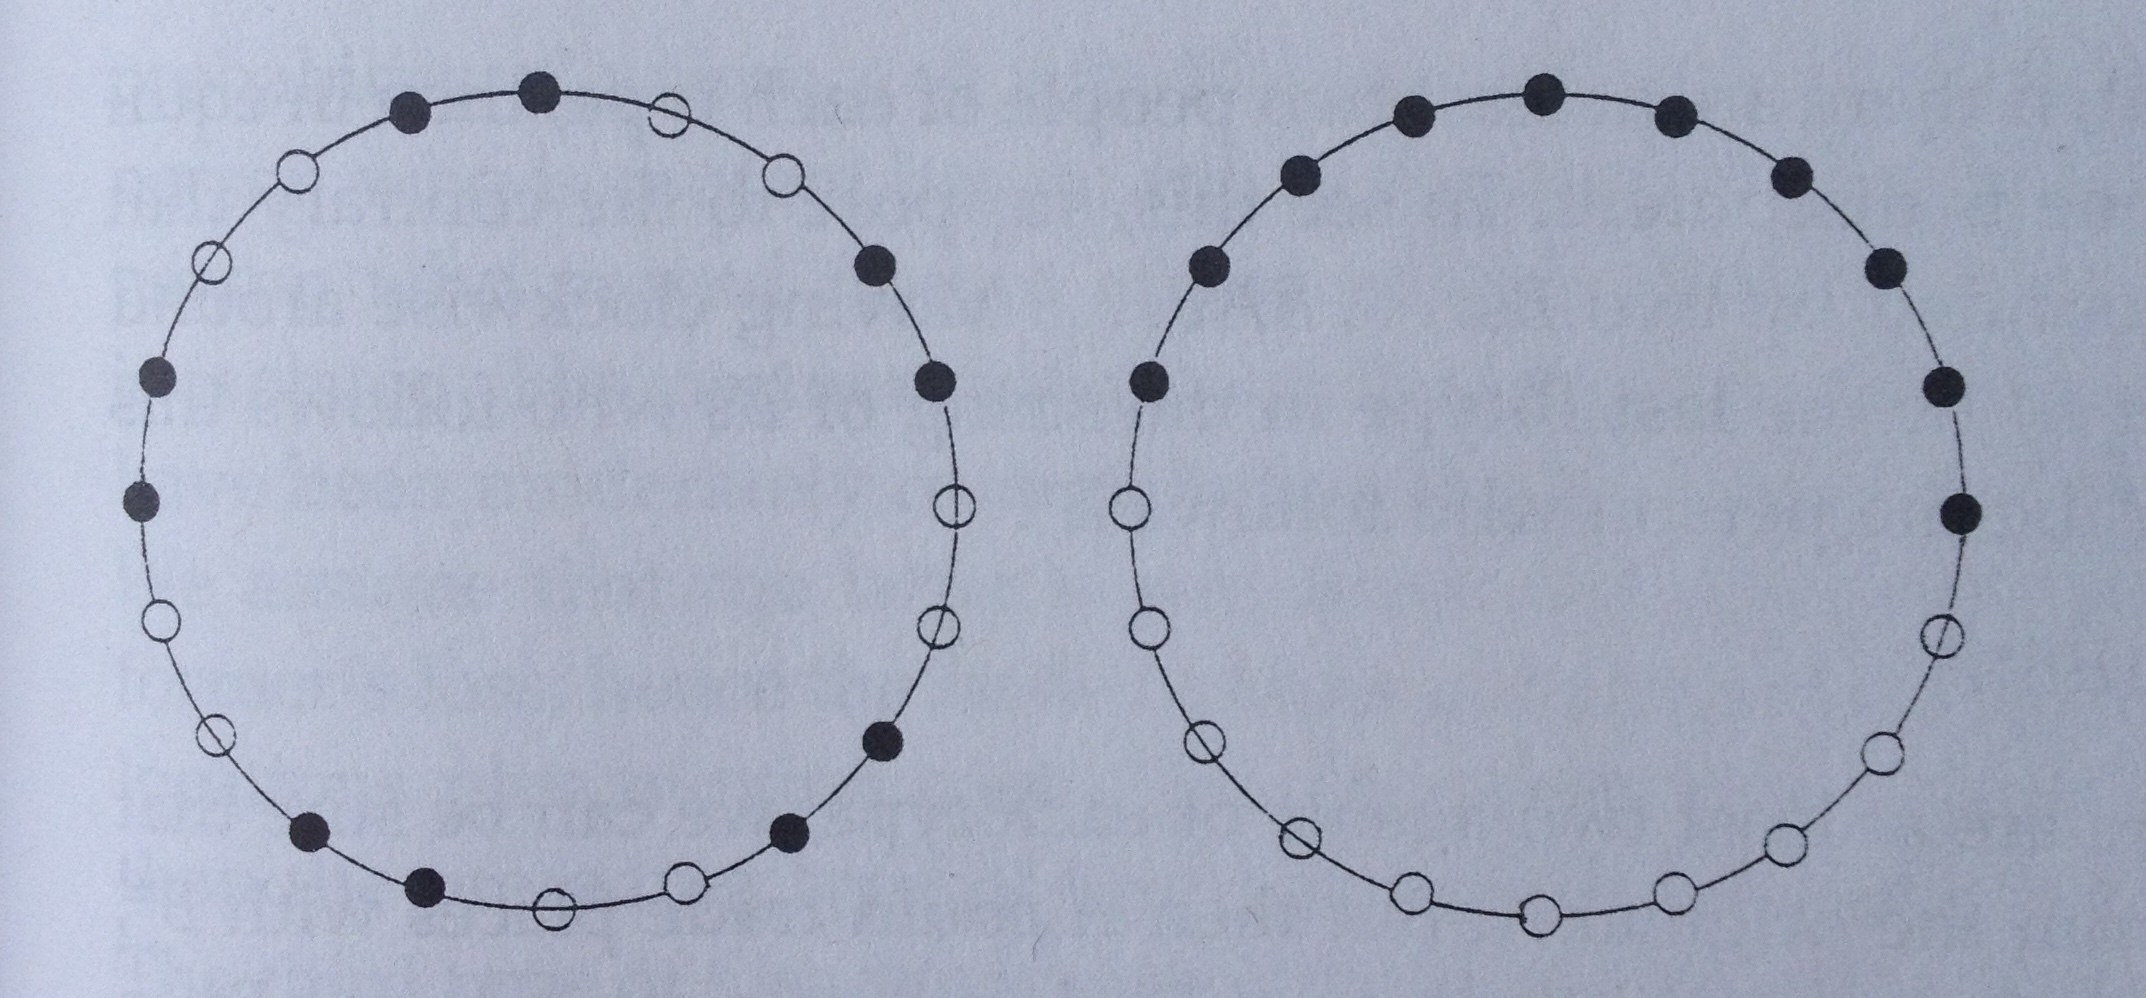
\includegraphics[scale=0.15]{YoungModel}
\caption{Completely integrated and completely segregated states}
\end{figure}

In Young’s model, an agent can be in one of the following three states:
\begin{itemize}
  \item \textit{discontent} -  if both neighbours are not like oneself
  \item \textit{moderately content} – if both neighbours are like oneself
  \item \textit{content} - if one neighbour is same type as oneself and the other neighbour is of different type
\end{itemize}

Young introduces a different rule to determine the agents’ movement than what we are going to see in Schelling’s model. Agents trade their places, but there is a cost associated with the movement so there is no incentive to trade unless the overall level of contentment is raised. Between two randomly selected agents we have an \textit{advantageous trade} if both individuals gain from trading places, otherwise we have a \textit{disadvantageous trade}. It is clear that we are talking about an advantageous trade if the trade is happening between two agents of different type.  

Young makes the following affirmation: from any initial configuration, there always exists some sequence of improving trades that leads to equilibrium. Furthermore, he states that the particular equilibrium that is reached depends on the order in which people have traded their positions, it is path dependent. 

In Schelling's model, agents have perfect logic, that is, they would not move if they were content or their position would not improve after moving. However, in Young's linear model we are introduced to agents who might make a trade for unexplained reasons. Young shows that if the probability of making idiosyncratic trades is small enough, the most likely form of spontaneous order is a completely segregated order. He states that "the segregated states are the only stochastically stable states". Schelling's derives a similar result using a slightly different model.

What is important to notice in Young's model is the fact that we started with a random distribution where nobody wanted to live in a neighbourhood made 100\% of people like oneself. In fact, everyone would prefer a perfectly integrated society. But, as we see from the results of the paper, segregated patterns are more likely to occur due to the cumulative impact of many agents which make a trading decision is locally optimal, but not globally so.




\subsubsection{The Schelling Model of Ethnic Residential Dynamics: Beyond the Integrated - Segregated Dichotomy of Patterns }

\textit{The Schelling Model of Ethnic Residential Dynamics: Beyond the Integrated - Segregated Dichotomy of Patterns} paper \cite[]{ethnic} tries to use the Schelling model to reproduce the ethnic residential patterns of Israeli people. The paper brings into the equation a new type of model pattern in which only a part of the group will segregate, while the rest will remain in their initial location even if their are discontent. All these patterns are compared with the patterns in the real cities, presenting and discussing the differences that occur. 

\begin{figure}[H]
\centering
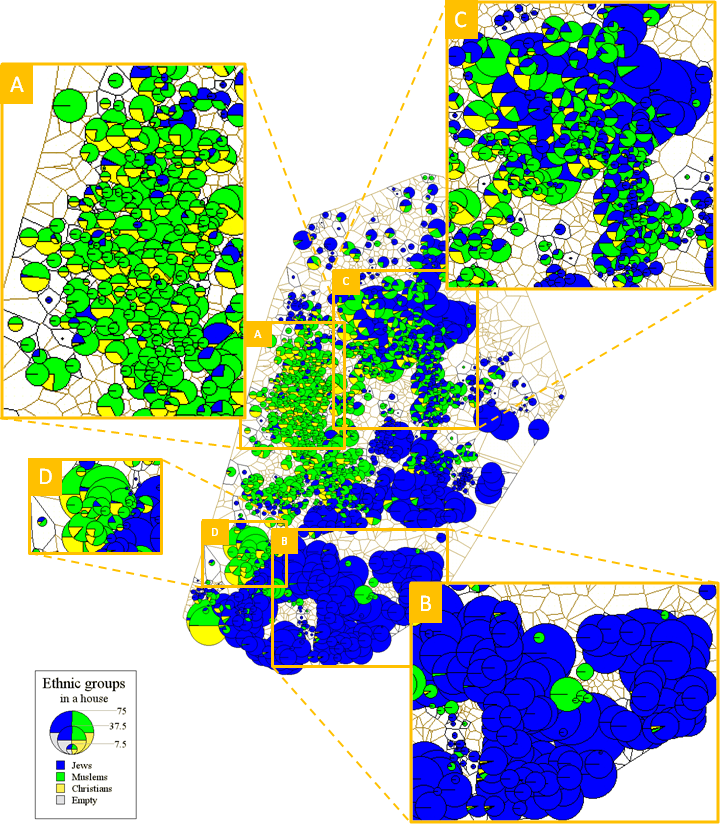
\includegraphics[scale=0.31]{Yaffo}
\caption{Ethnic residential distribution of Yaffo in 1995}
\end{figure}

\begin{figure}[H]
\centering
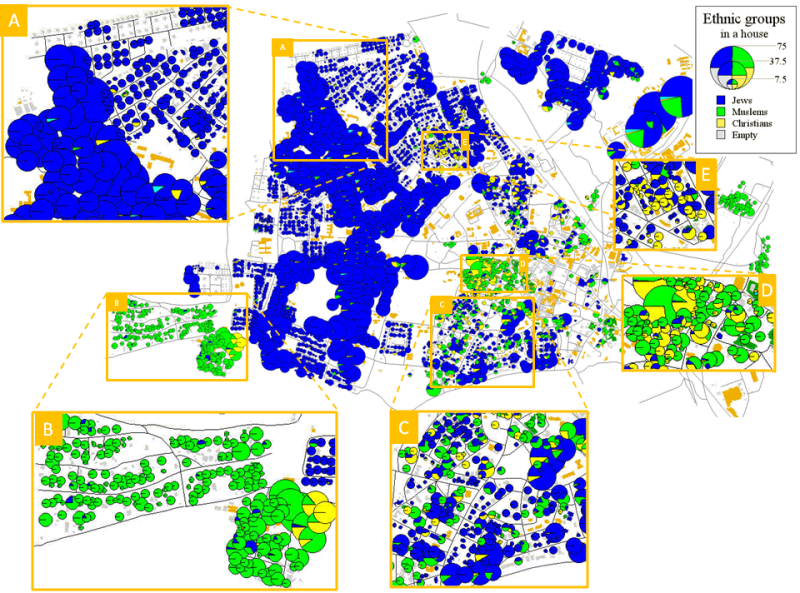
\includegraphics[scale=0.5]{Ramle}
\caption{Ethnic residential distribution of Ramle in 1995}
\end{figure}

\begin{figure}[H]
\centering
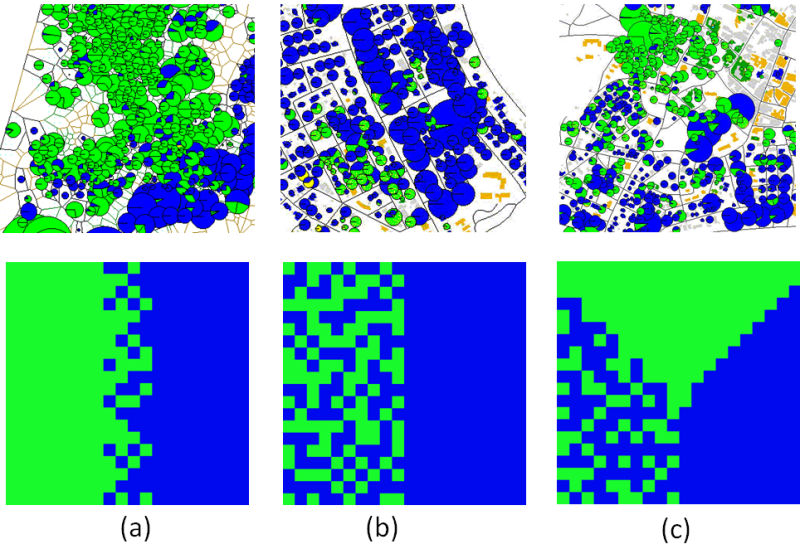
\includegraphics[scale=0.3]{compare}
\caption{Comparison of actual ethnic residential distribution with the model pattern}
\end{figure}

\subsubsection{A Wealth and Status-Based Model of Residential Segregation}
 Stephen Benard and Robb Willer in \textit{A Wealth and Status-Based Model of Residential Segregation}\cite[]{AWealthandStatus-BasedModelofResidentialSegregation} present an extension of Schelling's model by introducing some new factors to the model: the wealth and status of the agents and the desirability and affordability of the residences. The authors first look into how correlated the wealth and status are and how does the wealth of residents affect the affordability in that neighbourhood. 
 
 The results of the study show that the greater the correlation between wealth and status, the higher the chances of segregation, that is, little to no mixing between people with different wealth and status level in the final configuration. Furthermore, the change of the prices of the houses acts as a precondition for the status segregation.

\subsubsection{Parable of the Polygons }
Segregation is an important problem in present society and numerous scientists and designers have realised how important is to educate the population from a young age if a change is to be made in future. They designed different games to help students understand how segregation happens and how even a small local bias can lead to a global segregated society.

\textit{Parable of the Polygons} \cite[]{parable} is one of such playable games of Thomas Schelling's model of neighbourhood segregation. The creators of this game saw the importance of understanding Shelling's model in order to deal with segregation. They created a fun, easy to use game in order to help others understand how a small, personal bias could have a large-scale impact, over a whole society.

\begin{figure}[H]
\centering
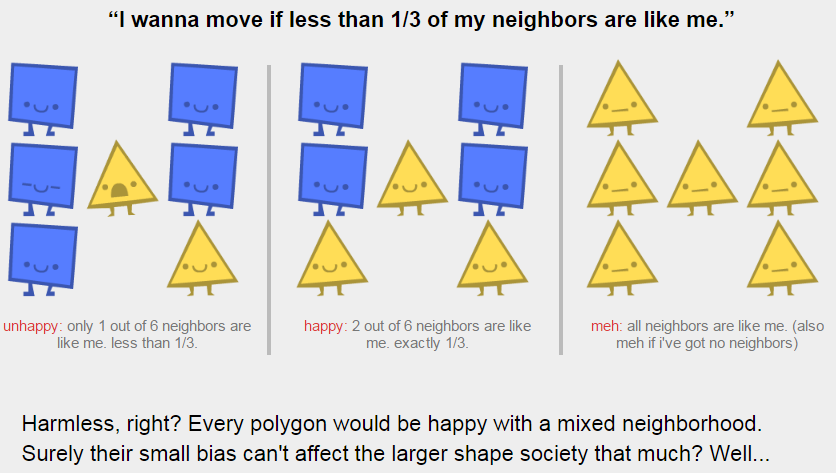
\includegraphics[scale=0.3]{parable1}
\caption{Helping the user understand how your personal bias might affect the larger neighbourhood}
\end{figure}

There are two very interesting points that are covered in this article. Firstly, even a small 33\% bias could have a significant impact over the society. Secondly, being in an already-segregated society, it turns out that it is almost impossible to go back to a mixed neighbourhood even if everyone would lower their preferences. The following figure shows that even if people lowered their expectation from 33\% to 10\%, nobody moves. \verb|i.e| Being a segregated society to start with, even if we all stop having any kind of ethnic bias, it will still take a long time to go back to a mixed distribution, if ever.

\begin{figure}[H]
\centering
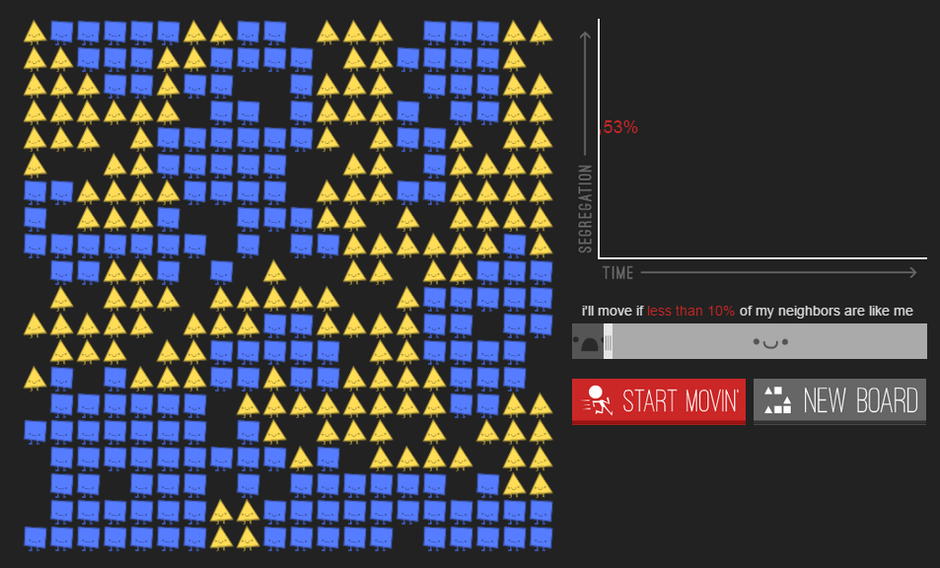
\includegraphics[scale=0.3]{parable2}
\caption{A 33\% preference lowered to 10\% still does not change the distribution}
\end{figure}


\subsection{Development environment}
So far, most multi-agent computational models out there are modeled using object oriented programs. Each agent's characteristics and behaviour are implemented in a class and an agent is an instantiation of the class. The environment rules (in our case would be the turn function) is defined in a different class. The complication with a model designed this way is the \textit{randomness} of the program. For example, in our model we would have to define a strict turn function. We are going to see later how same agent behaviour, but different turn functions can affect the final, resulting configuration. In other words, we get different outcomes depending of which player gets to move first. One could, of course, create a random turn function where each time a random agent is picked from the crowd. However, in normal object oriented programs it is complicated to ensure that everyone is being picked infinitely often.\\

In order to automatically test Schelling's linear model, and variations of the model with random turn functions we used \textbf{NuSMV}. To understand what \textit{NuSMV} is and how it works, we first have to talk about \textit{SMV} model checker, \textit{Binary Decision Trees} and \textit{Binary Decision Diagrams}.\\ \\

\textbf{SMV - Symbolic Model Checker}

When we refer to a \textbf{model checking} we talk about the following problem: Given a model of the system \verb|M| and a property (or specification) \verb|P|, we want to \textit{automatically} and \textit{exhaustively} check that \verb|M| meets \verb|P|. In other words, model checking is a technique to check automatically that a specification is met in a \textit{finite-state} system. The specifications about the system must be expressed as temporal logic formulas. Then, we use symbolic algorithms to traverse the model and check if the specifications work or not. \\

\textbf{Binary Decision Trees (BDTs)}

\textit{Binary Decision Trees} (BDTs) are a way of representing Boolean formulas just like truth tables. A BDT is a rooted, directed, acyclic graph which consists of several decision nodes and terminal nodes. Terminal nodes are labelled with 0 or 1 and all the non-terminal nodes are labelled with a Boolean variable. Each non-terminal node has exactly two outgoing edges: one labelled 0 and the other one labelled 1. \textit{Figure 7} shows an example of truth table and its corresponding BDT for the formula $ (\neg x_1 \land \neg x_2 \land \neg x_3) \lor (x_1 \land  x_2) \lor(x_2 \land  x_3) $. By convention, \textit{dashed} lines are used to represent that we assigned false to the variable and \textit{continuous} lines for when we assign the variable to true. 

\begin{figure}[ht]
\centering
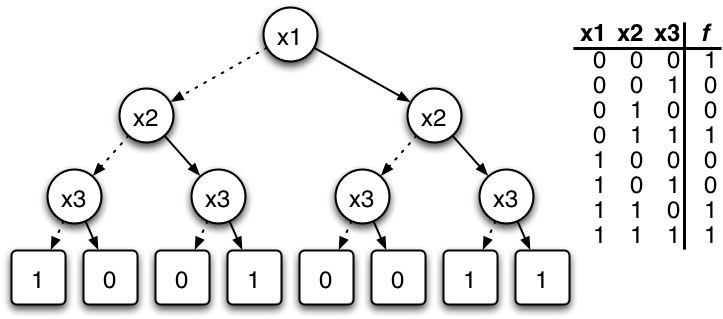
\includegraphics[scale=0.45]{BDD}
\caption{BDT and Truth Table for formula $ (\neg x_1 \land \neg x_2 \land \neg x_3) \lor (x_1 \land  x_2) \lor(x_2 \land  x_3) $ \cite[]{BDD_fig}}
\end{figure}

BDTs are preferred over Truth Tables since they are more compact and also, more importantly, performing a Boolean operation on the formula means that we have to recompute the entire truth table while we can do operations directly on BDTs rather quickly.\\


\textbf{Binary Decision Diagrams (BDDs)}

\textit{Binary Decision Diagrams} (BDDs) are more compact data structures than BDTs, also used to represent Boolean formulas. We can apply the following steps on a BDT to reduce the size and produce a BDD:
\begin{itemize}
    \item Sharing the terminal nodes of the BDT. In other words, we will have only two terminal nodes: a 0-node and a 1-node.
    \item Remove redundant decision points. That is, if both outgoing edges of a node \verb|e| point to the same node \verb|n|, remove \verb|e|.
    \item Remove duplicate non-terminals. If two distinct nodes of the BDD are the roots to two structurally identical subBDDs the remove one of the nodes (and its subBDD) and send all the incoming edges to the other one.
\end{itemize}
After applying all the steps above to the BDT, the result will be a \textit{Reduced} BDD. 

\begin{figure}[ht]
\centering
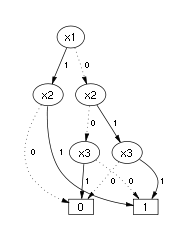
\includegraphics[scale=0.85]{ROBDD}
\caption{ROBDD for formula $ (\neg x_1 \land \neg x_2 \land \neg x_3) \lor (x_1 \land  x_2) \lor(x_2 \land  x_3) $ \cite[]{ROBDD}}
\end{figure}


\textit{Figure 8} shows the resulting Reduced BDD for the above formula $ (\neg x_1 \land \neg x_2 \land \neg x_3) \lor (x_1 \land  x_2) \lor(x_2 \land  x_3) $.


We say that a BDD is \textit{ordered} if different variables appear in the same order on all paths from the root. It is important to note that we can represent sets and functions between sets as Boolean formulas. Hence, OBDDs are used to perform symbolic model checking since we can create a OBDD representing a Boolean formula. Functions and operations on sets can be executed on the OBDD. Another important property of a OBDD is the fact that their reduced structure is unique.\\




\textbf{NuSMV Model Checker}

A \textit{model checker} is a tool that provides a programming language to describe the model succinctly and it performs the check automatically against some given specifications. 

\textit{NuSMV} is an extended version of the symbolic model checker \verb|SMV|. The input language of NuSMV is simply called SMV and the properties that we want to check in SMV  are formulae in LTL (Linear Temporal Logic)\cite[]{LTL} and CTL (Computational Tree Logic) \cite[]{CTL}. Given the model as an input and a property, NuSMV will return true if the property holds in that model, false otherwise. If the answer is false, NuSMV generates a counter-example.


NuSMV is based on Binary Decision Diagrams (\textit{BDDs}).This was a suitable tool for the task because for any given initial configuration it would generate a binary decision diagram generating this way all the possible final configuration, considering all the possible turn functions. Furthermore, we can introduce \textit{Fairness constraints} such that each agent is going to be picked infinitely often. It allows us to answer questions such as "Does the configuration converge for all possible turn functions?" or "How segregated the final configurations are?". We are going to explain what all these mean and why they are important in the \textit{Formal Analysis} chapter. \\ 

\textbf{Python}

A downside of the SMV language is the fact that it does not support control flow statements, such as  \textit{for-loops}. Therefore, in order to generate the model in an \verb|smv| file, we used a Python \cite[]{Python} script. This way, passing in the initial configuration, we can create the model of the system in SMV, together with the properties that we want to check. Thus, the generated file can be run using NuSMV. The SMV model of the system is explained in detail in the \textit{Simulation} chapter. There, we explain how the modules are generated and how they work.

\end{document}